\documentclass{techrep}
%%%%%%%%%%%%%%%%%%%%%%%%%%%%%%%%%%%%%%%%%%%%%%%%%%%%%
%
%  Definition Starts
%
%%%%%%%%%%%%%%%%%%%%%%%%%%%%%%%%%%%%%%%%%%%%%%%%%%%%%
 
\usepackage{amsfonts}
\usepackage{amsthm}

\newcommand{\centeripe}[1]{\begin{center}\Ipe{#1}\end{center}}
\newcommand{\comment}[1]{}

\newcommand{\centerpsfig}[1]{\centerline{\psfig{#1}}}

\newcommand{\seclabel}[1]{\label{sec:#1}}
\newcommand{\Secref}[1]{Section~\ref{sec:#1}}
\newcommand{\secref}[1]{\mbox{Section~\ref{sec:#1}}}

\newcommand{\alglabel}[1]{\label{alg:#1}}
\newcommand{\Algref}[1]{Algorithm~\ref{alg:#1}}
\newcommand{\algref}[1]{\mbox{Algorithm~\ref{alg:#1}}}

\newcommand{\applabel}[1]{\label{app:#1}}
\newcommand{\Appref}[1]{Appendix~\ref{app:#1}}
\newcommand{\appref}[1]{\mbox{Appendix~\ref{app:#1}}}

\newcommand{\tablabel}[1]{\label{tab:#1}}
\newcommand{\Tabref}[1]{Table~\ref{tab:#1}}
\newcommand{\tabref}[1]{Table~\ref{tab:#1}}

\newcommand{\figlabel}[1]{\label{fig:#1}}
\newcommand{\Figref}[1]{Figure~\ref{fig:#1}}
\newcommand{\figref}[1]{\mbox{Figure~\ref{fig:#1}}}

\newcommand{\eqlabel}[1]{\label{eq:#1}}
%\renewcommand{\eqref}[1]{(\ref{eq:#1})}
\newcommand{\myeqref}[1]{(\ref{eq:#1})}
\newcommand{\Eqref}[1]{Equation~(\ref{eq:#1})}

\newtheorem{theorem}{Theorem}{\bfseries}{\itshape}
\newcommand{\thmlabel}[1]{\label{thm:#1}}
\newcommand{\thmref}[1]{Theorem~\ref{thm:#1}}

\newtheorem{lemma}{Lemma}{\bfseries}{\itshape}
\newcommand{\lemlabel}[1]{\label{lem:#1}}
\newcommand{\lemref}[1]{Lemma~\ref{lem:#1}}

\newtheorem{conj}{Conjecture}{\bfseries}{\itshape}
\newcommand{\conjlabel}[1]{\label{lem:#1}}
\newcommand{\conjref}[1]{Conjecture~\ref{lem:#1}}

\newtheorem{corollary}{Corollary}{\bfseries}{\itshape}
\newcommand{\corlabel}[1]{\label{cor:#1}}
\newcommand{\corref}[1]{Corollary~\ref{cor:#1}}

\newtheorem{obs}{Observation}{\bfseries}{\itshape}
\newcommand{\obslabel}[1]{\label{obs:#1}}
\newcommand{\obsref}[1]{Observation~\ref{obs:#1}}

\newtheorem{clm}{Claim}{\bfseries}{\itshape}
\newcommand{\clmlabel}[1]{\label{clm:#1}}
\newcommand{\clmref}[1]{Claim~\ref{clm:#1}}

\newtheorem{assumption}{Assumption}{\bfseries}{\rm}
\newenvironment{ass}{\begin{assumption}\rm}{\end{assumption}}
\newcommand{\asslabel}[1]{\label{ass:#1}}
\newcommand{\assref}[1]{Assumption~\ref{ass:#1}}

\newcommand{\proclabel}[1]{\label{alg:#1}}
\newcommand{\procref}[1]{Procedure~\ref{alg:#1}}

\theoremstyle{definition}

\newtheorem{definition}{Definition}
\newcommand{\deflabel}[1]{\label{rem:#1}}
\newcommand{\defref}[1]{Definition~\ref{rem:#1}}


\newtheorem{rem}{Remark}
\newcommand{\remlabel}[1]{\label{rem:#1}}
\newcommand{\remref}[1]{Remark~\ref{rem:#1}}

\newtheorem{lesson}{Lesson}
\newcommand{\leslabel}[1]{\label{les:#1}}
\newcommand{\lesref}[1]{Lesson~\ref{les:#1}}

\newtheorem{op}{Open Problem}
\newcommand{\oplabel}[1]{\label{op:#1}}
\newcommand{\opref}[1]{Open Problem~\ref{op:#1}}
\newtheorem{prb}{Problem}{\bfseries}{\rm}

\theoremstyle{plain}

\newcommand{\etal}{et al.}

\newcommand{\keywords}[1]{\noindent\textbf{Keywords:} #1}
\newcommand{\voronoi}{Vorono\u\i}
\newcommand{\ceil}[1]{{\lceil #1 \rceil}}
\newcommand{\Ceil}[1]{{\left\lceil #1 \right\rceil}}
\newcommand{\floor}[1]{{\lfloor #1 \rfloor}}
\newcommand{\Floor}[1]{{\left\lfloor #1 \right\rfloor}}
\newcommand{\R}{\mathbb{R}}
\newcommand{\N}{\mathbb{N}}
\newcommand{\Z}{\mathbb{Z}}
\newcommand{\Sp}{\mathbb{S}}
\newcommand{\E}{\mathrm{E}}
\newcommand{\DD}{\ensuremath{\mathcal{D}}}


\usepackage{verbatim}
\usepackage{algorithm2e}
\usepackage[utf8]{inputenc}
\usepackage{microtype}
\usepackage{amsthm,amsmath,graphicx}
\usepackage{caption}
\usepackage{subcaption}
\usepackage[letterpaper]{hyperref}
\usepackage[table,dvipsnames]{xcolor}
\definecolor{linkblue}{named}{Blue}
\hypersetup{colorlinks=true, linkcolor=linkblue,  anchorcolor=linkblue,
	citecolor=linkblue, filecolor=linkblue, menucolor=linkblue,
	urlcolor=linkblue} 
\setlength{\parskip}{1ex}
\usepackage{wasysym}
\usepackage{graphicx}
\usepackage{caption}
\usepackage{enumitem}
\usepackage{thmtools, thm-restate}
\usepackage{wrapfig}
%\usepackage{mathrsfs}
\usepackage{float}
\usepackage{stackrel}
\usepackage{fixfoot}
\usepackage[utf8]{inputenc}
\usepackage[english]{babel}
\usepackage{mathrsfs}  
\usepackage{venturis}
\usepackage{placeins}

\listfiles

%\graphicspath{{./graphics/}}%helpful if your graphic files are in another directory

\newtheorem{thm}{Theorem}
\newtheorem{lem}[thm]{Lemma}

\newcommand{\notes}[1]{\marginpar{\tiny{#1}}}

\newlength\problemsep
\setlength\problemsep{10pt}
\newcommand{\given}{}
\newcommand{\find}{}
\newcommand{\nogo}{\textsc{impossible}}
\newcommand{\go}{\textsc{possible}}
%\newcommand{\bdry}[1]{\ensuremath{\textsl{bd}\  #1}}
\newcommand{\bdP}{\ensuremath{\partial P}}
%\newcommand{\bdPccw}[1]{\ensuremath{\bdP^{ccw}(#1)}}
\newcommand{\bdPccw}[1]{\ensuremath{\partial^{+}(#1)}}
\newcommand{\bdPcw}[1]{\ensuremath{\partial^{-}(#1)}}
\newcommand{\ERCW}[1]{\ensuremath{R_{\textsl{cw}}( #1 )}}
\newcommand{\ERCCW}[1]{\ensuremath{R_{\textsl{ccw}}( #1 )}}
%\newcommand{\ERSPLIT}[1]{\ensuremath{R_{\textsl{split}}( #1 )}}
\newcommand{\ERSPLIT}[1]{\ensuremath{S( #1 )}}
\newcommand{\vangle}[1]{\ensuremath{u_{#1}}}
\newcommand{\vanglecw}[1]{\ensuremath{u_{#1}^{\textsl{\tiny cw}}}}
\newcommand{\vangleccw}[1]{\ensuremath{u_{#1}^{\textsl{\tiny ccw}}}}
%\newcommand{\vangleccw}[1]{\ensuremath{w_{#1 (ccw)}}}
\newcommand{\accumccw}[1]{\ensuremath{\textsl{accum}^{\textsl{\tiny ccw}}(#1)}}
\newcommand{\accumcw}[1]{\ensuremath{\textsl{accum}^{\textsl{\tiny cw}}(#1)}}
\newcommand{\pifrac}[2]{\ensuremath{\frac{#1 \pi}{#2}}}
\newcommand{\piover}[1]{\pifrac{}{#1}}
\newcommand{\piovertwo}{\ensuremath{\frac{\pi}{2}}}
\newcommand{\threepiovertwo}{\ensuremath{\frac{3\pi}{2}}}
\newcommand{\tqpi}{\pifrac{3}{4}}
\newcommand{\sed}[1]{\ensuremath{D(#1)}}
\newcommand{\bd}[1]{\ensuremath{\partial D(#1)}}



\newenvironment{problem}[1] {			% the typesetting here needs work.
	\vspace{\problemsep}
	\noindent{\scshape \underline{#1}}
	\renewcommand\descriptionlabel[1]%
		{\hspace{\labelsep}\textsc{##1}}
	\renewcommand{\given}{\item[Given:]}
	\renewcommand{\find}{\item[Find:]}
	\begin{description}
}{
	\end{description}
	\vspace{\problemsep}
}

%\newcommand{\jit}[1]{\textcolor{blue}{Jit: #1}}
\newcommand{\jit}[1]{}
\newcommand{\tom}[1]{\textcolor{teal}{Tom: #1}}

\bibliographystyle{abbrv}

%%%%%%%%%%%%%%%%%%%%%%%%%%%%%%%%%%%%%%%%%%%%%%%%%%%%%
%
%  Definitions over
%
%%%%%%%%%%%%%%%%%%%%%%%%%%%%%%%%%%%%%%%%%%%%%%%%%%%%%



\usepackage{graphicx} % Required for inserting images

\title{Polynomial multiplication using NTT}
%\author{Navjeet Sandhu}
%\date{September 2024}

\begin{document}

\maketitle

\section{Introduction}
The Number Theoretic Transform (NTT) can efficiently calculate polynomial multiplication using the convolution theorem with a quasi-linear complexity instead of $O(d^2)$

\section{Linear convolution}
Suppose that $g(x)$ and $h(x)$ are polynomials of degree $d - 1$ and $x$ is the polynomial variable. Polynomial multiplication equals a discrete linear convolution between the coefficients’ vectors g and h. The traditional multiplication algorithm has an $O(d^2)$ complexity.

\begin{align*}
 y[k] &= (g*h)[k] \\
        &= \sum_{i=0}^{k}g[i]h[k-i] \\
\end{align*} 

\subsection{Example}
If $g(x) = 1 + 2x + 3x^2 + 4x^3$ and $h(x) = 5 + 6x + 7x^2 + 8x^3$ or in vector notation:  $g = [1, 2, 3, 4]$, and $h = [5, 6, 7, 8]$. The linear convolution result is $y(x) = 5 + 16x + 34x^2 + 60x^3 + 61x^4 + 52x^5 + 32x^6$, or in vector notation, $y = [5, 16, 34, 60, 61, 52, 32]$.

\begin{figure}[H]
 	\centering
 	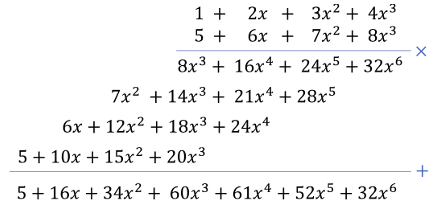
\includegraphics[width=.7\columnwidth]{fig/trad_mult.png}
 	\caption{The traditional multiplication} 
\label{fig:TradMult}
\end{figure}

\begin{figure}[H]
 	\centering
 	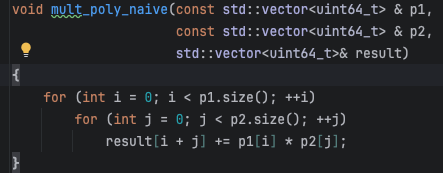
\includegraphics[width=.8\columnwidth]{fig/naive_poly_mult.png}
 	\caption{The traditional multiplication in C++} 
\label{fig:naive_poly_mult}
\end{figure}


\section{Integer ring modulo $\Z_{q}$}
An integer ring modulo q (also called integers modulo a prime number), denoted by $\Z_{q}$, is a mathematical structure known as a cyclic group or finite field in abstract algebra. Specifically, it is the set of residue classes of integers modulo q. This means it's the set of all possible remainders when integers are divided by q.
For example, if q equals 2, then $\Z_{q}$ (which is $\Z_{2}$ in this case) includes only 0 and 1 because any integer either leaves a remainder of 0 or 1 when divided by 2. In the field of cryptography, we typically work with finite fields. The exciting thing about working in a finite field is that the polynomial coefficients “wrap around” when multiplied. So, regardless of how much polynomial arithmetic we perform, the polynomial coefficients can still be bounded in a fixed range, which is very attractive from an implementation perspective.

\begin{figure}[H]
 	\centering
 	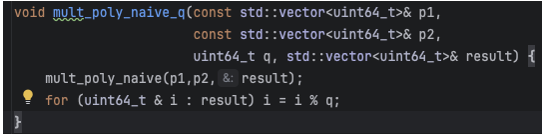
\includegraphics[width=.9\columnwidth]{fig/Zq_Cplus.png}
 	\caption{Integer ring modulo $\Z_{q}$ in C++} 
\label{fig:Zq_Cplus}
\end{figure}


\subsection{Example}
If q equals 17, then $\Z_{q}$ (which is $\Z_{17}$ in this case) includes only 0 to 16 because any integer leaves a remainder of 0 to 16 when divided by 17. Hence the vector multiplication for vectors $g = [1, 2, 3, 4]$, and $h = [5, 6, 7, 8]$ with modulo a prime number $q = 17$ is  $[5, 16, 0, 9, 10, 1, 15]$

\section{Positive wrapped convolution (cyclic convolution)}
However, one can quickly notice an item that is not so positive in the current setting - the degree of the polynomial will only grow larger and larger as we perform more multiplications. That means we need a more extended array to store coefficients and more complex convolutions every time a multiplication is performed. It would be great if the degree of the polynomials could “wrap around” just like the coefficients. As it turns out, another algebraic structure is precisely for that - Polynomial Quotient Rings. Like in the base field  $\Z_{q}$, where we would take modulo q after every arithmetic operation, we can also take modulo some polynomial $\Phi(x)$ after every polynomial operation. The resulting polynomial’s degree would never be more significant or equal to the degree of $\Phi(x)$. We call such structure $\Z_{q}[x]/(\Phi(x))$. In the context of lattice-based Cryptography, $\Phi(x)$ is chosen to be a polynomial looking either like $x^d - 1$ or $x^d + 1$.  A cyclic convolution or positive wrapped convolution, $PWC(x)$ is defined as: $PWC(x) = \Z_{q}/x^d - 1$


\begin{figure}[H]
 	\centering
 	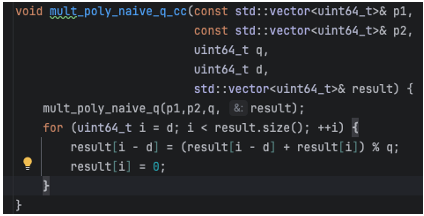
\includegraphics[width=.9\columnwidth]{fig/PWC_cplus.png}
 	\caption{Positive wrapped convolution (cyclic convolution) in C++} 
\label{fig:PWC_cplus}
\end{figure}



\subsection{Example}
If $g(x) = 1 + 2x + 3x^2 + 4x^3$ and $h(x) = 5 + 6x + 7x^2 + 8x^3$ or in vector notation:  $g = [1, 2, 3, 4]$, and $h = [5, 6, 7, 8]$. We already have calculated the linear convolution result is $y(x) = 5 + 16x + 34x^2 + 60x^3 + 61x^4 + 52x^5 + 32x^6$, or in vector notation, $y = [5, 16, 34, 60, 61, 52, 32]$. If we don't apply an integer ring modulo q, then $PWC(x) = y(x)$ mod $x^d - 1$.  We need a long division by $x^d - 1$ to calculate positive wrapped convolution. Thus, the result of the cyclic convolution is $PWC(x) = 66 + 68x + 66x^2 + 60x^3$ or $[66, 68, 66, 60]$. Notice that we present the result sorted in increasing power.


\begin{figure}[H]
 	\centering
 	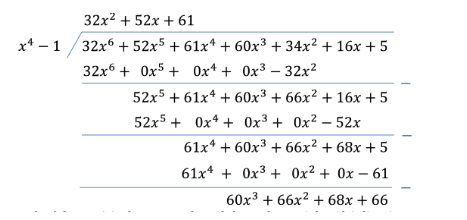
\includegraphics[width=.7\columnwidth]{fig/PWC_1.png}
 	\caption{Schoolbook method for positive wrapped convolution (cyclic convolution)} 
\label{fig:PWC_1}
\end{figure}

\section{Negative wrapped convolution (negacyclic convolution)}
A cyclic convolution or negative wrapped convolution, $NWC(x)$ is defined as: $PWC(x) = \Z_{q}/x^d + 1$  

\begin{figure}[H]
 	\centering
 	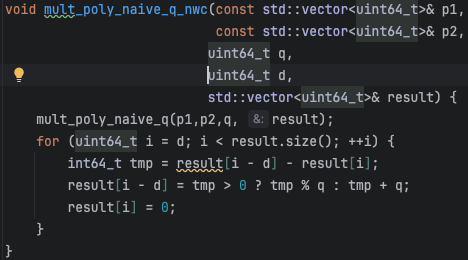
\includegraphics[width=.9\columnwidth]{fig/NWC_cplus.png}
 	\caption{Negative wrapped convolution (negacyclic convolution) in C++} 
\label{fig:NWC_cplus}
\end{figure}

\subsection{Example}
If $g(x) = 1 + 2x + 3x^2 + 4x^3$ and $h(x) = 5 + 6x + 7x^2 + 8x^3$ or in vector notation:  $g = [1, 2, 3, 4]$, and $h = [5, 6, 7, 8]$. We already have calculated the linear convolution result is $y(x) = 5 + 16x + 34x^2 + 60x^3 + 61x^4 + 52x^5 + 32x^6$, or in vector notation, $y = [5, 16, 34, 60, 61, 52, 32]$. If we don't apply an integer ring modulo q, then $NWC(x) = y(x)$ mod $x^d + 1$.  We need a long division by $x^d + 1$ to calculate positive wrapped convolution. Thus, the result of the negacyclic convolution is $NWC(x) = -56 -36x + 2x^2 + 60x^3$ or $[-56, -36, 2, 60]$. Notice that we present the result sorted in increasing power.

\begin{figure}[H]
 	\centering
 	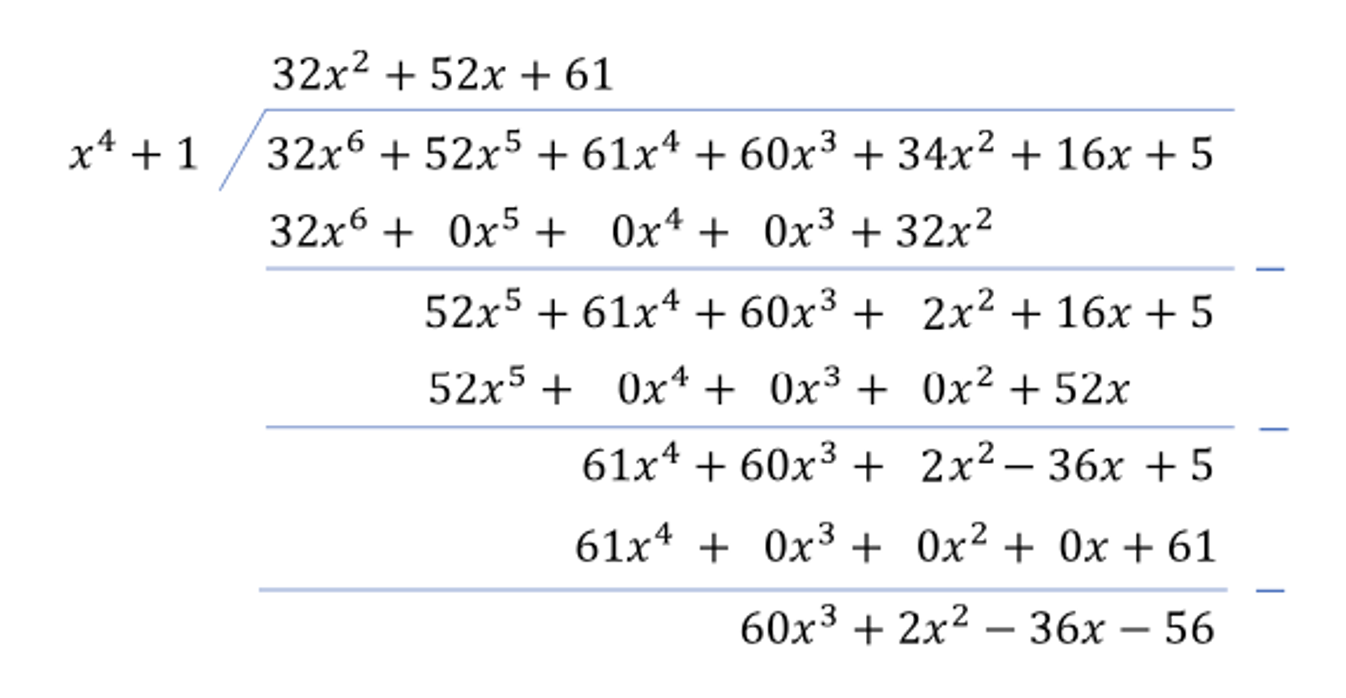
\includegraphics[width=.7\columnwidth]{fig/NWC_1.png}
 	\caption{Schoolbook method for negative wrapped convolution (negacyclic convolution)} 
\label{fig:NWC_1}
\end{figure}


\section{NTT-Based Convolutions}
In this section, we present the basics of NTT-based convolutions.

\subsection{Congruence}
The symbol $\equiv$ denotes congruence and is different from equality. While equality means that items are the same, congruence means items have the same remainder when divided by mod. In a ring $\Z_{7681}$  and $d = 4$, the 4-th root of unity, which satisfy the condition $\omega^4 \equiv 1$ mod $7681$ are ${3383, 4298, 7680}$

\subsection{Primitive n-th Root of Unity}
Let $\Z_{q}$  be an integer ring modulo q, and $d - 1$ is the polynomial degree of g(x) and h(x). $\omega$ is a primitive n-th root of unity in $\Z_{q}$ if and only if:
$\omega^d \equiv 1$ mod $q$ and $\omega^k \nequiv 1$ mod $q$  for $k < d$. 

\subsection{Example}
In a ring $\Z_{7681}$  and $d = 4$, the 4-th root of unity, which satisfy the condition $\omega^4 \equiv 1$ mod $7681$ are ${3383, 4298, 7680}$. Out of three roots, 7680 is not a primitive n-th root of unity, as there exists k = 2 < d that satisfy $\omega^d \equiv 1$ mod $7691$ Therefore $\omega$ = 3383 or $\omega$ = 4298 are the primitive 4-th root of unity in $\Z_{7681}$. The value of $\omega$  will be important in calculating NTT and positive-wrapped convolution.

\subsection{Primitive 2n-th Root of Unity}
Let $\Z_{q}$  be an integer ring modulo q, and $d - 1$ is the polynomial degree of g(x) and h(x) and $\omega$ is a primitive n-th root. $\psi$ is a primitive 2n-th root of unity in $\Z_{q}$ if and only if:
$\psi^2 \equiv \omega$ mod $q$ and $\psi^d \equiv {-1}$ mod $q$. 

\subsection{Example}

In a ring $\Z_{7681}$, $d = 4$, and $\omega$ = 3383, the 2n-th root of unity, which satisfies the above conditions, are 1925 and 5756 as $1925^2 = 5756^2 \equiv 3383$ mod 7681 and $1925^4$ = $5756^4$ = $7680 \equiv -1$ mod 7681. The value of $\psi$  will be significant in calculating NTT and negative-wrapped convolution.

\section{NTT-Based Positive-Wrapped Convolution}
The NTT of a polynomial does not have any physical meaning, unlike Discrete Fourier Transform (DFT) which represents a signal in the frequency domain. However, NTT preserves one of the essential properties of DFT: the convolution theorem, which is valuable in calculating polynomial multiplication.

\subsection{NTT Based on $\omega$}
The Number Theoretic Transform (NTT) of a vector of polynomial coefficients a is defined as $\hat{a}$ = NTT(a), where:

$\quad \quad \quad \hat{a_j} = \sum_{i=0}^{d - 1}\omega^{ij}a_i$ mod q

and j = 0, 1, 2, . . . , d - 1

\subsection{Example}

If $g(x) = 1 + 2x + 3x^2 + 4x^3$ or in vector notation:  $g = [1, 2, 3, 4]$. 
In a ring $\Z_{7681}$, $d = 4$ and $\omega =3383$. Thus, the NTT of $g$ can be calculated by the following matrix multiplication:


\begin{figure}[H]
 	\centering
 	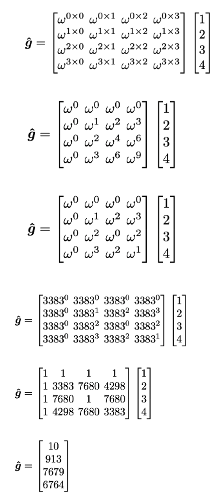
\includegraphics[width=.4\columnwidth]{fig/NTT_cal.png}
 	\caption{NTT calculations example} 
\label{fig:NTT_cal}
\end{figure}

Therefore, the NTT(g) = $\hat{g}$ = [10, 913, 7679, 6764] in $\Z_{7681}$, $d = 4$ and $\omega =3383$. Note that the NTT of a particular polynomial is not always unique. It depends on the choice of $\omega$. The NTT result will differ if one uses $\omega$ = 4298 instead of $\omega$ = 3383. 


\subsection{INTT Based on $\omega$}
The Inverse of Number Theoretic Transform (INTT) of an NTT vector $\hat{a}$ is defined as a = NTT($\hat{a}$), where:

$\quad \quad \quad a_i = d^{-1}\sum_{i=0}^{d - 1}\omega^{-ij}\hat{a}_j$ mod q

and j = 0, 1, 2, . . . , d - 1

Note that the INTT has a formula that is very similar to NTT. The only differences are $\omega$ replaced by its inverse in $\Z_{q}$. It always holds that a = INTT(NTT(a)).

\subsection{Example}

If NTT(g) = $\hat{g}$ = $[10, 913, 7679, 6764]$. In a ring $\Z_{7681}$, $d = 4$ and $\omega =3383$. Thus, the INTT of $\hat{g}$ can be calculated by the following matrix multiplication:


\begin{figure}[H]
 	\centering
 	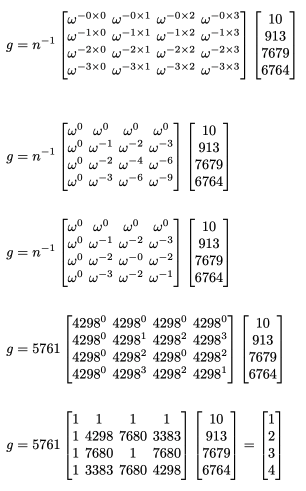
\includegraphics[width=.4\columnwidth]{fig/INTT_cal.png}
 	\caption{INTT calculations example} 
\label{fig:INTT_cal}
\end{figure}

In the figure above $n^{-1}$ = $d^{-1}$ = $4^{-1}$ = 5761 after applying mod 7681. Therefore, the INTT($\hat{g}$) = g = [1, 2, 3, 4], which is the initial polynomial coefficient given  

\subsection{Using NTT to Calculate Positive-Wrapped Convolutions}

Because NTT is a variant of DFT in the polynomial ring, one can apply DFT convolution theorem to calculate positive-wrapped convolution. Let g and h are the multiplicands’ vectors of polynomial coefficients. The positive-wrapped convolution of g and h, PWC can be calculated by:
PWC = INTT(NTT(g) $\circ$ NTT(h))

where $\circ$ is an element-wise vector multiplication in $\Z_{q}$.

\subsection{Example}
Let g = [1,2,3,4] and h = [5,6,7,8]. The NTT of them are $\Z_{7681}$ are ($\hat{g}$) = $[10, 913, 7679, 6764]$ and ($\hat{h}$) = $[10, 913, 7679, 6764]$ when $\omega =3383$. We can calculate their positive-wrapped convolution by:

\begin{figure}[H]
 	\centering
 	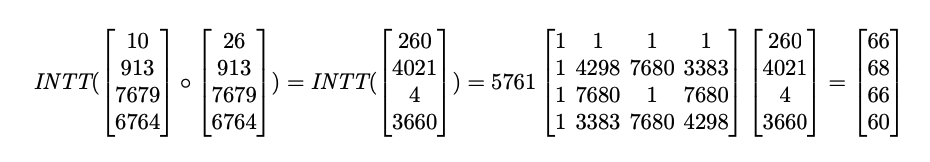
\includegraphics[width=.9\columnwidth]{fig/PWC_NTT.png}
 	\caption{Using NTT to Calculate PWC} 
\label{fig:PWC_NTT}
\end{figure}

PWC = $[66, 68, 66, 60]$, the same result as calculated by schoolbook multiplication and long division 



\section{NTT-Based Negative-Wrapped Convolution}
This section explains the definition of Number Theoretic Transform (NTT) and its inverse (INTT) based on the 2n-th root of unity, $\psi$.

\subsection{NTT Based on $\psi$}
The Number Theoretic Transform (${NTT}^\psi$) of a vector of polynomial coefficients a is defined as $\hat{a}$ = ${NTT}^\psi$(a), where:

$\quad \quad \quad \hat{a_j} = \sum_{i=0}^{d - 1}\psi^{2ij+i}a_i$ mod q

\subsection{Example}

If $g(x) = 1 + 2x + 3x^2 + 4x^3$ or in vector notation:  $g = [1, 2, 3, 4]$. 
In a ring $\Z_{7681}$, $d = 4$ and $\psi =1925$. Thus, the matrix multiplication using the above equation can calculate the ${NTT}^\psi$ of $g$.

${NTT}^\psi$(g) = $\hat{g}$ = $[1467, 2807, 3471, 7621]$. 

\subsection{INTT Based on $\psi$}
The Inverse of the Number Theoretic Transform (INTT) of an NTT vector $\hat{a}$ is defined as a = ${INTT}^\psi$($\hat{a}$), where:

$\quad \quad \quad a_i = d^{-1}\sum_{i=0}^{d - 1}\psi^{-(2ii+j)j}\hat{a}_j$ mod q

and j = 0, 1, 2, . . . , d - 1

\subsection{Example}

Let ${NTT}^\psi$(g) = $\hat{g}$ = $[1467,2807,3471,7621]$. In a ring $\Z_{7681}$, $d = 4$, $\omega =3383$ and $\psi =1925$. Thus, the INTT of $\hat{g}$ can be calculated by matrix multiplication. In the equation $d^{-1}$ = $4^{-1}$ = 5761 and $/psi^{-1}$ = ${1925}^{-1}$ = 1213. Therefore, the INTT($\hat{g}$) = g = [1, 2, 3, 4], which is the initial polynomial coefficient given  

\subsection{Using NTT to Calculate Negative-Wrapped Convolutions}

Let g and h are the multiplicands vectors of polynomial coefficients. The negative-wrapped convolution of g and h, NWC can be calculated by:
NWC = ${INTT}^\psi$(${NTT}^\psi$(g) $\circ$ ${NTT}^\psi$(h))

where $\circ$ is an element-wise vector multiplication in $\Z_{q}$.

\subsection{Example}
Let g = [1,2,3,4] and h = [5,6,7,8]. The ${NTT}^\psi$ of them are ($\hat{g}$) = $[1467,2807,3471,7621]$ and ($\hat{h}$) = $[2489,7489,6478,6607]$. In a ring$\Z_{7681}$, $\omega =3383$ and $\psi =1925$. NWC = $[7625, 7645, 2, 60]$, the same result calculated by schoolbook multiplication and long division when written with negative numbers [-56, -36, 2, 60].

\end{document}

